\documentclass[times]{G7-32} % стиль и язык

\sloppy

% Настройки стиля ГОСТ 7-32
% Для начала определяем, хотим мы или нет, чтобы рисунки и таблицы нумеровались в пределах раздела, или нам нужна сквозная нумерация.
\EqInChapter % формулы будут нумероваться в пределах раздела
\TableInChapter % таблицы будут нумероваться в пределах раздела
\PicInChapter % рисунки будут нумероваться в пределах раздела

\renewcommand{\DefinesIntro}{В настоящей выпускной квалификационной работе магистра применяют следующие сокращения и обозначения:}

% Добавляем гипертекстовое оглавление в PDF
\usepackage[
bookmarks=true, colorlinks=true, unicode=true,
urlcolor=black,linkcolor=black, anchorcolor=black,
citecolor=black, menucolor=black, filecolor=black,
]{hyperref}

\AfterHyperrefFix

\usepackage{microtype}% полезный пакет для микротипографии, увы под xelatex мало чего умеет, но под pdflatex хорошо улучшает читаемость

% Тире могут быть невидимы в Adobe Reader
\ifInvisibleDashes
\MakeDashesBold
\fi

\usepackage{graphicx}   % Пакет для включения рисунков

% С такими оно полями оно работает по-умолчанию:
% \RequirePackage[left=20mm,right=10mm,top=20mm,bottom=20mm,headsep=0pt,includefoot]{geometry}
% Если вас тошнит от поля в 10мм --- увеличивайте до 20-ти, ну и про переплёт не забывайте:
\geometry{right=15mm}
\geometry{left=30mm}
\geometry{bottom=20mm}
\geometry{ignorefoot}% считать от нижней границы текста


% Пакет Tikz
\usepackage{tikz}
\usetikzlibrary{arrows,positioning,shadows}

% Произвольная нумерация списков.
\usepackage{enumerate}

% ячейки в несколько строчек
\usepackage{multirow}

% itemize внутри tabular
\usepackage{paralist,array}

%\setlength{\parskip}{1ex plus0.5ex minus0.5ex} % разрыв между абзацами
\setlength{\parskip}{1ex} % разрыв между абзацами
\usepackage{blindtext}

% Центрирование подписей к плавающим окружениям
%\usepackage[justification=centering]{caption}

\usepackage{newfloat}
\DeclareFloatingEnvironment[
placement={!ht},
name=Equation
]{eqndescNoIndent}
\edef\fixEqndesc{\noexpand\setlength{\noexpand\parindent}{\the\parindent}\noexpand\setlength{\noexpand\parskip}{\the\parskip}}
\newenvironment{eqndesc}[1][!ht]{%
    \begin{eqndescNoIndent}[#1]%
\fixEqndesc%
}
{\end{eqndescNoIndent}}
 % остальные стандартные настройки убраны в preamble.inc.tex
% Математика
\usepackage{mathtools, cancel, physics, euscript, xfrac, amsmath, amsthm}

\newtheorem{Th}{Теорема}
\newtheorem{Lm}{Лемма}
\newtheorem{Df}{Определение}
\newtheorem{Ex}{Пример}
\newtheorem{Rm}{Ремарка}
\newtheorem{Alg}{Алгоритм}
\newtheorem{Ax}{Аксиома}
\newtheorem{Crl}{Следствие}
\newtheorem{Prp}{Гипотеза}


% Настройки листингов.
\ifPDFTeX
% 8 Листинги

\usepackage{listings}

% Значения по умолчанию
\lstset{
  basicstyle= \footnotesize,
  breakatwhitespace=true,% разрыв строк только на whitespacce
  breaklines=true,       % переносить длинные строки
%   captionpos=b,          % подписи снизу -- вроде не надо
  inputencoding=koi8-r,
  numbers=left,          % нумерация слева
  numberstyle=\footnotesize,
  showspaces=false,      % показывать пробелы подчеркиваниями -- идиотизм 70-х годов
  showstringspaces=false,
  showtabs=false,        % и табы тоже
  stepnumber=1,
  tabsize=4,              % кому нужны табы по 8 символов?
  frame=single
}

% Стиль для псевдокода: строчки обычно короткие, поэтому размер шрифта побольше
\lstdefinestyle{pseudocode}{
  basicstyle=\small,
  keywordstyle=\color{black}\bfseries\underbar,
  language=Pseudocode,
  numberstyle=\footnotesize,
  commentstyle=\footnotesize\it
}

% Стиль для обычного кода: маленький шрифт
\lstdefinestyle{realcode}{
  basicstyle=\scriptsize,
  numberstyle=\footnotesize
}

% Стиль для коротких кусков обычного кода: средний шрифт
\lstdefinestyle{simplecode}{
  basicstyle=\footnotesize,
  numberstyle=\footnotesize
}

% Стиль для BNF
\lstdefinestyle{grammar}{
  basicstyle=\footnotesize,
  numberstyle=\footnotesize,
  stringstyle=\bfseries\ttfamily,
  language=BNF
}

% Определим свой язык для написания псевдокодов на основе Python
\lstdefinelanguage[]{Pseudocode}[]{Python}{
  morekeywords={each,empty,wait,do},% ключевые слова добавлять сюда
  morecomment=[s]{\{}{\}},% комменты {а-ля Pascal} смотрятся нагляднее
  literate=% а сюда добавлять операторы, которые хотите отображать как мат. символы
    {->}{\ensuremath{$\rightarrow$}~}2%
    {<-}{\ensuremath{$\leftarrow$}~}2%
    {:=}{\ensuremath{$\leftarrow$}~}2%
    {<--}{\ensuremath{$\Longleftarrow$}~}2%
}[keywords,comments]

% Свой язык для задания грамматик в BNF
\lstdefinelanguage[]{BNF}[]{}{
  morekeywords={},
  morecomment=[s]{@}{@},
  morestring=[b]",%
  literate=%
    {->}{\ensuremath{$\rightarrow$}~}2%
    {*}{\ensuremath{$^*$}~}2%
    {+}{\ensuremath{$^+$}~}2%
    {|}{\ensuremath{$|$}~}2%
}[keywords,comments,strings]

% Подписи к листингам на русском языке.
\renewcommand\lstlistingname{Листинг}
\renewcommand\lstlistlistingname{Листинги}

\else
\usepackage{local-minted}
\fi

% Любимые команды
\newcommand{\Code}[1]{\textbf{#1}}
 % полезные макросы листингов


%\NirEkz{Экз. 3}                                  % Раскоментировать если не требуется
%\NirGrif{Секретно}                % Наименование грифа

%\gosttitle{Gost7-32}       % Шаблон титульной страницы, по умолчанию будет ГОСТ 7.32-2001, 
% Варианты GostRV15-110 или Gost7-32 
 
\NirOrgLongName{Министерство общего и профессионального образования \\
Российской Федерации\par
ГОСУДАРСТВЕННЫЙ ТЕХНИЧЕСКИИ УНИВЕРСИТЕТ
}                                           %% Полное название организации

% \NirUdk{УДК № 378.14}
% \NirGosNo{№ госрегистрации 01970006723}
%\NirInventarNo{Инв. № ??????}

%\NirConfirm{Согласовано}                  % Смена УТВЕРЖДАЮ
\NirBoss[.49]{Проректор университета\\по научной работе}{И.И. Иванов}            %% Заказчик, утверждающий НИР


%\NirReportName{Научно-технический отчет}   % Можно поменять тип отчета
%\NirAbout{О составной части \par опытно-конструкторской работы} %Можно изменить о чем отчет

%\NirPartNum{Часть}{1}                      % Часть номер

%\NirBareSubject{}                  % Убирает по теме если раскоментить

% \NirIsAnnotacion{АННОТАЦИОННЫЙ }         %% Раскомментируйте, если это аннотационный отчёт
%\NirStage{промежуточный}{Этап \No 1}{} %%% Этап НИР: {номер этапа}{вид отчёта - промежуточный или заключительный}{название этапа}
%\NirStage{}{}{} %%% Этап НИР: {номер этапа}{вид отчёта - промежуточный или 

\Nir{Социально-экономические проблемы подготовки военных специалистов\\в гражданских вузах России}

\NirSubject{ФЕМИНИЗАЦИЯ АРМИИ КАК СОЦИАЛЬНЫЙ ПРОЦЕСС}                                   % Наименование темы
%\NirFinal{}                        % Заключительный, если закоментировать то промежуточный
%\finalname{итоговый}               % Название финального отчета (Заключительный) 
%\NirCode{Шифр\,---\,САПР-РЛС-ФИЗТЕХ-1} % Можно задать шифр как в ГОСТ 15.110
\NirCode{}

\NirManager{Зам. проректора по научной работе}{И.И. Иванов} %% Название руководителя
\NirIsp{Руководитель темы}{И.И. Иванов} %% Название руководителя

\NirYear{2023}%% если нужно поменять год отчёта; если закомментировано, ставится текущий год
\NirTown{Москва}                           %% город, в котором написан отчёт
 % стиль титульного листа и заголовки

\begin{document}

\frontmatter % выключает нумерацию ВСЕГО; здесь начинаются ненумерованные главы: реферат, введение, глоссарий, сокращения и прочее.

\maketitle % создает титульную страницу

\begin{executors}
    \personalSignature{Первый исполнитель}{ФИО}
    \personalSignature{Второй исполнитель}{ФИО}
\end{executors}

%\listoffigures % список рисунков

%\listoftables % список таблиц

%\NormRefs % нормативные ссылки 
% Команды \breakingbeforechapters и \nonbreakingbeforechapters
% управляют разрывом страницы перед главами.
% По-умолчанию страница разрывается.

% \nobreakingbeforechapters
% \breakingbeforechapters

\Referat

Выпускная квалификационная работа магистра состоит из \pageref{LastPage}\,стр.%
\ifnum \totfig >0
, \totfig~рис.%
\fi
\ifnum \tottab >0
, \tottab~табл.%
\fi
%
\ifnum \totbib >0
, \totbib~источн.%
\fi
%
\ifnum \totapp >0
, \totapp~прил.%
\else
.%
\fi

Данный опус, как и более новые версии этого документа, можно взять по адресу (\url{https://github.com/afaikiac/latex-g7-32}). Шаблон соответствует ГОСТ-у настолько хорошо насколько это смогли сделать авторы оригинального репозитория и люди работавшие над этим форком.

Текст в документе носит совершенно абстрактный характер.


\tableofcontents

\printnomenclature % автоматический список сокращений

\Introduction

Добавлять пункты в "{}Термины и определения"{} и "{}Перечень сокращений и обозначений"{} можно где угодно в коде. Команда \verb|\Define| добавляет пункт в первый список, \verb|\Abbrev| добавляет пункт во второй список. 

Проверяем как у нас работают сокращения, обозначения и определения "---
MAX,
\Abbrev{MAX}{maximum "--- максимальное значение параметра}
API
\Abbrev{API}{application programming interface "--- внешний интерфейс взаимодействия с приложением}
с обратным прокси.
\Define{Обратный прокси}{тип прокси-сервера, который ретранслирует}


\mainmatter % это включает нумерацию глав и секций в документе ниже

\chapter{Аналитический раздел}
\label{cha:analysis}


В данном разделе анализируется и классифицируется существующая всячина и рассматриваются способы создания новой всячины.

\section{Анализ того и сего}

В работе можно использовать разделы \verb|\chapter|, \verb|\section|, подразделы \verb|\subsection|, подподраздела \verb|\subsubsection| и параграфа \verb|\paragraph|. Однако, следует помнить, что разделы разрешены только в основной части работы. Во введении, заключении и других структурных элементах они запрещены. Старайтесь избегать случаев, когда в разделе существует только один подраздел.

\subsection{Пример использования подраздела}
\subsubsection{Пример использования подподраздела}

\paragraph{Проверка} параграфа. Вроде работает.
\paragraph{Вторая проверка} параграфа. Опять работает.

\begin{itemize}
\item Это список с палочками. 
\item Хотя он соответствует требованиям ГОСТ, лучше использовать список с номерами, чтобы облегчить чтение.
\end{itemize}

\subsection{Пример использования блок-схемы}

\subsubsection*{Заголовки разделов}

В работе можно использовать и подподпункты, например \verb|\subsubsection|. Однако, лучше не нумеровать этот уровень разделов, чтобы не усложнять структуру документа.

\section{Подсистема всякой ерунды}

Существует несколько подсистем, среди которых можно выделить:

\begin{enumerate}
\item Перечисление с номерами.
\item Нумерация первого уровня. В соответствии с ГОСТ, первый уровень нумеруется буквами, а на втором уровне "--- цифрами. Элементы на первом уровне выравниваются как обычные абзацы. Проверим теперь вложенные списки.
\begin{enumerate}
\item Нумерация второго уровня.
\item Нумерация второго уровня. Проверяем на очень длинной строке, чтобы убедиться, что выравнивание работает правильно.
\end{enumerate}
\item По мнению Лукьяненко, человеческий мозг старается свести любую проблему к выбору из трех вариантов.
\item Четвертый (и последний) элемент списка.
\end{enumerate}

\chapter{Конструкторский раздел}
\label{cha:design}

В данном разделе проектируется новая всячина.

\section{Архитектура всячины}

Используйте окружение \verb|figure| для создания изображений. Код ниже является стандартным и его следует копировать каждый раз, когда необходимо вставить новое изображение.

Команда \verb|\includegraphics|, находящаяся внутри окружения, непосредственно вставляет изображение, единственный ее аргумент "--- путь до изображения. Используйте параметр \verb|scale| для изменения размера изображения. Команда \verb|\caption| задает подпись под изображением, а команда \verb|\label| задает уникальный идентификатор объекта, на который можно ссылаться в тексте.

\begin{figure}[ht]
    \centering
    \includegraphics[scale=0.5]{example-image-a}
    \caption{Подпись к изображению}
    \label{fig:example_fig_1}
\end{figure}

\begin{figure}[ht]
    \centering
    \includegraphics[scale=1.5,angle=90]{example-image}
    \caption{Большой рисунок}
\end{figure}

Кстати, про изображения. Во-первых, для изображений следует использовать \verb|[ht]|. Если после этого изображения все еще вставляются "{}не по ГОСТ"{}, т.е. слишком далеко от места ссылки, "--- значит, у вас \textbf{слишком мало текста}! Хотя и ужасный параметр \verb|ht!| у окружения \texttt{figure} тоже никто не отменял, но его использование делает документ страшным, как в Word. Поэтому просьба не использовать его, если это возможно.

\section{Существующие подходы к созданию всячины}

В отчетах может быть необходимо использовать таблицы "--- см. табл.~\ref{tab:tabular} и~\ref{tab:longtable}. Для создания небольших таблиц можно использовать окружение \verb|tabular| внутри окружения \verb|table| (последнее полностью аналогично окружению \verb|figure|, но добавляет другую подпись). Для более продвинутых таблиц можно обратиться к информации на сайте \url{https://www.overleaf.com/learn/latex/Tables}. Там вы найдете советы по созданию сложных таблиц, но они не слишком сложные.

\begin{table}[ht]
  \caption{Пример короткой таблицы с коротким названием}
  \begin{tabular}{|r|c|c|c|l|}
  \hline
  Тело      & $F$ & $V$  & $E$ & $F+V-E-2$ \\
  \hline
  Тетраэдр  & 4   & 4    & 6   & 0         \\
  Куб       & 6   & 8    & 12  & 0         \\
  Октаэдр   & 8   & 6    & 12  & 0         \\
  Додекаэдр & 20  & 12   & 30  & 0         \\
  Икосаэдр  & 12  & 20   & 30  & 0         \\
  \hline
  Эйлер     & 666 & 9000 & 42  & $+\infty$ \\
  \hline
  \end{tabular}
  \label{tab:tabular}
\end{table}

Для создания больших таблиц следует использовать пакет \verb|longtable|, который позволяет создавать таблицы на несколько страниц в соответствии с требованиями ГОСТ.

Для того, чтобы длинный текст разбивался на несколько строк в пределах одной ячейки, необходимо использовать формат ячейки \texttt{p} и явно указывать ее ширину в мм/дюймах (\texttt{110mm}), относительно ширины страницы (\texttt{0.22\textbackslash textwidth}), и т.п.

Можно также использовать уменьшенный шрифт, но, пожалуйста, не забывайте применять его ко всей таблице сразу.

\begin{center}
  \begin{longtable}{|p{0.40\textwidth}|c|p{0.30\textwidth}|}
    \caption{Пример длинной таблицы с длинным названием на много длинных-длинных строк}
    \label{tab:longtable}
    \\ \hline
    Вид шума & Громкость, дБ & Комментарий \\
    \hline \endfirsthead
    \subcaption{Продолжение таблицы~\ref{tab:longtable}}
    \\ \hline \endhead
    \hline \subcaption{Продолжение на след. стр.}
    \endfoot
    \hline \endlastfoot
    Порог слышимости             & 0     &                                                \\
    \hline
    Шепот в тихой библиотеке     & 30    &                                                \\
    Обычный разговор             & 60-70 &                                                \\
    Звонок телефона              & 80    & \small{Конечно, это было до эпохи мобильников} \\
    Уличный шум                  & 85    & \small{(внутри машины)}                        \\
    Гудок поезда                 & 90    &                                                \\
    Шум электрички               & 95    &                                                \\
    \hline
    Порог здоровой нормы         & 90-95 & \small{Длительное пребывание на более
    громком шуме может привести к ухудшению слуха}                                        \\
    \hline
    Мотоцикл                     & 100   &                                                \\
    Power Mower                  & 107   & \small{(модель бензокосилки)}                  \\
    Бензопила                    & 110   & \small{(Doom в целом вреден для здоровья)}     \\
    Рок-концерт                  & 115   &                                                \\
    \hline
    Порог боли                   & 125   & \small{feel the pain}                          \\
    \hline
    Клепальный молоток           & 125   & \small{(автор сам не знает, что это)}          \\
    \hline
    Порог опасности              & 140   & \small{Даже кратковременное пребывание на
    шуме большего уровня может привести к необратимым последствиям}                       \\
    \hline
    Реактивный двигатель         & 140   &                                                \\
                                 & 180   & \small{Необратимое полное повреждение
                                 слуховых органов}                                        \\
    Самый громкий возможный звук & 194   & \small{Интересно, почему?..}                   \\
  \end{longtable}
\end{center}

\chapter{Технологический раздел}
\label{cha:impl}

В данном разделе описано изготовление и требование всячины. Кстати,
в Latex нужно эскейпить подчёркивание (писать <<\verb|some\_function|>> для \Code{some\_function}).

\ifPDFTeX
% TODO: сделать рабочее решение для листингов c русским текстом в pdflatex
\else

Для вставки кода есть пакет \texttt{minted}. Он хорош всем кроме: необходимости Python (есть во всех нормальных (нет, Windows, я не про тебя) ОС) и Pygments и того, что нормально работает лишь в \XeLaTeX.

\ifdefined\NoMinted
Но к сожалению, у вас, по-видимому, не установлен Python или pygmentize.
\else
Можно пользоваться расширенным BFN:

\begin{listing}[H]
\begin{ebnfcode}
 letter = "A" | "B" | "C" | "D" | "E" | "F" | "G"
       | "H" | "I" | "J" | "K" | "L" | "M" | "N"
       | "O" | "P" | "Q" | "R" | "S" | "T" | "U"
       | "V" | "W" | "X" | "Y" | "Z" ;
digit = "0" | "1" | "2" | "3" | "4" | "5" | "6" | "7" | "8" | "9" ;
symbol = "[" | "]" | "{" | "}" | "(" | ")" | "<" | ">"
       | "'" | '"' | "=" | "|" | "." | "," | ";" ;
character = letter | digit | symbol | "_" ;
 
identifier = letter , { letter | digit | "_" } ;
terminal = "'" , character , { character } , "'" 
         | '"' , character , { character } , '"' ;
 
lhs = identifier ;
rhs = identifier
     | terminal
     | "[" , rhs , "]"
     | "{" , rhs , "}"
     | "(" , rhs , ")"
     | rhs , "|" , rhs
     | rhs , "," , rhs ;
 
rule = lhs , "=" , rhs , ";" ;
grammar = { rule } ;
\end{ebnfcode}
\caption{EBNF определённый через EBNF}
\label{lst:ebnf}
\end{listing}

А вот в листинге \ref{lst:c} на языке C работают русские комменты. Спасибо Pygments и Minted за это.

\begin{listing}[H]
\cfile{res/code/test.c}
\caption{Пример — test.c} 
\end{listing}
\label{lst:c}

\fi
\fi

\chapter{Экспериментальный раздел}
\label{cha:research}

Математическая формула может встречаться в тексте: $E = mc^2$. Для больших формул следует использовать окружение \verb|equation|:
\begin{equation}\label{eq:f1}
    E = mc^2.
\end{equation}
На формулу можно сослаться, например, так: (\ref{eq:f1}). См. также раздел \ref{cha:econom}. Использование других окружений для формул, таких как двойные доллары или скобки:
\[
    E = mc^2,
\]
не рекомендуется из-за отсутствия нумерации.

В конце больших формул следует ставить подходящий знак препинания в соответствии с контекстом: точку, запятую, точку с запятой или ничего.

Согласно ГОСТ, каждое новое обозначение, вводимое в формуле, должно быть пояснено сразу после неё. Например:
\begin{equation}
    E = mc^2,
\end{equation}
где $m$ "--- масса, $c$ "--- скорость света.

Несколько примеров:

Формула с текстом:
\begin{equation}
    50 \text{ яблок} \times 100 \text{ яблок} =
    \textbf{ много яблок}
\end{equation}

Различные буквы и шрифты:
\begin{equation}
    \alpha,  \beta,  \gamma, \Gamma, \pi, \Pi, \phi, \varphi, \mu, \Phi, \xi, \zeta;
\end{equation}
\begin{equation}
    \mathbf M, \mathcal C, \mathbb R, \sin \theta = \mathrm{sin} \theta.
\end{equation}

Скобки:
\begin{equation}
    ( a ), [ b ], \{ c \}, | d |, \| e \|, \langle f \rangle, \lfloor g \rfloor, \lceil h \rceil, \ulcorner i \urcorner;
\end{equation}
\begin{equation}
    \left( a + b \right) \left[ 1 - \frac{b}{a+b} \right] = a;
\end{equation}
\begin{equation}
    \sqrt{|xy|} \leq \left| \frac{x + y}{2} \right|;
\end{equation}
\begin{equation}
    \int_a^b u \dv[2]{v}{x} \dd x = \left. u \dv{v}{x} \right|_a^b -\int_a^b \dv{u}{x} \dv{v}{x} \dd x;
\end{equation}
\begin{equation}
    \tilde f(\omega) = \frac{1}{2\pi} \int_{-\infty}^\infty f(x)e^{-i\omega x} \dd x;
\end{equation}
\begin{equation}
    \dot{\vec \omega} = \vec r_c \times \vec I;
\end{equation}
\begin{equation}
    u = \frac{-y}{x^2 + y^2}, \quad v = \frac{x}{x^2 + y^2}, \quad \text{и} \quad w = 0.
\end{equation}

Последовательности:
\begin{equation}
    (1+x)^n = \sum_{i=0}^n \binom{n}{i} x^i;
\end{equation}
\begin{equation}
    e^x = 1 + x + \frac{x^2}{2} + \frac{x^3}{6} + \cdots = \sum_{n \ge 0} \frac{x^n}{n!};
\end{equation}

Дроби:
\begin{equation}
    x = 
    a_0 + \frac{1}{a_1 + \frac{1}{a_2 + \frac{1}{a_3 + a_4}}}
    =
    a_0 + \frac{1}{\displaystyle a_1
        + \frac{1}{\displaystyle a_2
        + \frac{1}{\displaystyle a_3 + a_4}}}.
\end{equation}

Матрицы:
\begin{equation}
    \begin{pmatrix}
        1 & x & 0 \\
        0 & 1 & -1
    \end{pmatrix}
    \begin{pmatrix}
        1  \\
        y  \\
        1
    \end{pmatrix}
    =
    \begin{pmatrix}
        1 + xy  \\
        y - 1
    \end{pmatrix},
    \quad\quad
    \left(
    \begin{matrix}
        2 & 3 & 4\\
        5 & 6 & 7\\
        8 & 9 & 10
    \end{matrix}
    \right)
    v = 0;
\end{equation}
\begin{equation}
    \frac{n!}{k!(n-k)!} = \binom{n}{k};
\end{equation}
\begin{equation}
    \deg A =
    \left|
    \begin{matrix}
        -2 & 1 & 0 & 0 & \cdots & 0  \\
        1 & -2 & 1 & 0 & \cdots & 0  \\
        0 & 1 & -2 & 1 & \cdots & 0  \\
        0 & 0 & 1 & -2 & \ddots & \vdots \\
        \vdots & \vdots & \vdots & \ddots & \ddots & 1  \\
        0 & 0 & 0 & \cdots & 1 & -2
    \end{matrix}
    \right|.
\end{equation}

Фигурная скобка для нескольких случаев:
\begin{equation}
    |x| =
    \begin{cases}
        x, & x \ge 0, \\
        -x, & x< 0.
    \end{cases}
\end{equation}

Формулы в несколько строк:
\begin{align}
    F &= \{ F_{x} \in F_{c} \mid (|S| > |C|) \\
      &\wedge (\mathrm{minPixels} < |S| < \mathrm{maxPixels}) \\
      &\wedge (|S_{\mathrm{conected}}| > |S| - \epsilon) \}
\end{align}
или
\begin{multline}
    A_0 = \frac{1}{(\alpha + t_x)^{r + s + x}}{}_2 F_1 \left( r + s + x, x + 1; r + s + x + 1; \frac{\alpha - \beta}{\alpha + t_x} \right) \\
    \quad - \frac{1}{(\alpha + T)^{r + s + x}}{}_2 F_1 \left( r + s + x, x + 1; r + s + x + 1; \frac{\alpha - \beta}{\alpha + T} \right).
\end{multline}

Логика, доказательства:
\begin{equation}
    (\forall \varepsilon > 0) (\exists N \in \mathbb Z^+) (\forall n \ge N) (|x_n - a| < \varepsilon \iff \lim_{n \to +\infty} x_n = a);
\end{equation}
\begin{equation}
    A \implies B, \quad A \iff B, \quad A = \{z \in \mathbb Z \mid z = \bar z \};
\end{equation}
\begin{equation}
    f: X \to Y, \quad f: x \overset{F}{\mapsto} 5x \cos(\tfrac{\pi x}{2})
\end{equation}
\begin{equation}
    \frac{\cancel{\sqrt 2} \sin(x + 2)}{\cancel{2 \cdot \cos(\sfrac{\pi}{4})} \sin(x)} = \frac{\sin(x + 2)}{\sin(x)}, \quad \cancelto{0}{\sin(0)} \equiv 0.
\end{equation}

\section{Определения и теоремы}

В ГОСТе не представлены инструкции по оформлению определений и теорем. Однако в мировой практике принято следующее стилевое решение, которое можно использовать и в дипломной работе:

\begin{Df}[Метрическое пространство]\label{df:example}
    Метрическим пространством называют пару $(S; \rho)$, где для функции-\textit{метрики} $\rho: S \to \mathbb R^+$, если верно следующие три условия:
    \begin{enumerate}
        \item $a \in S : \rho(a, a) = 0$,
        \item $a, b \in S : \rho(a, b) = \rho(b, a)$,
        \item $a, b, c \in S : \rho(a, b) + \rho(b, c) \ge \rho(a, c)$.
    \end{enumerate}
\end{Df}

\begin{Th}[Хаусдорф]\label{th:example}
    В полном метрическом пространстве множество является компактом тогда и только тогда, когда оно замкнуто и вполне ограничено.
\end{Th}
\begin{proof}
    Текст доказательства.
\end{proof}

\begin{Ex}
    Множество вещественных чисел $\mathbb R$ с заданной на нём метрикой $\rho(a, b) = |a - b|$ формируют метрическое пространство.
\end{Ex}
\begin{proof}
    Следует из определения \ref{df:example}.
\end{proof}

Аналогично картинкам и таблицам, на определения, теоремы и другие блоки можно ссылаться при помощи команды \verb|\ref|: например, на теорему \ref{th:example}.

\chapter{Организационно-экономический раздел}
\label{cha:econom}

Интернет-ссылки оформляются как \url{https://www.google.com/}. Ссылка на картинку, формулу и другие объекты происходит при помощи команды \verb|\ref|: см. рис. \ref{fig:example_fig_1}. На ссылку можно кликнуть и перейти к объекту, на который она ссылается. Ссылка может быть как до объекта, так и после него. Обычно, для удобства, идентификатор начинают с префикса <<\verb|fig:|>> для рисунков, <<\verb|tab:|>> для таблиц, <<\verb|eq:|>> для формул, для <<\verb|section:|>> для разделов, <<\verb|th:|>> для теорем и так далее. Пример ссылки на раздел: см. раздел \ref{cha:research}. 

По условиям ГОСТ-а, на каждую картинку и таблицу должна присутствовать в тексте хотя бы одна ссылка. Желательно рядом с картинкой. Ссылка должна быть оформлена в духе "{}В соответствии с рисунком (таблицей, разделом) 2"{}.

Информация об цитируемых источниках хранится в файлах формата \verb|*.bib|. В этом проекте есть пример такого файла \verb|references.bib|. Похож на формат \verb|json|, но им не является. Заполняйте как можно больше полей там. Сразу готовую запись можно получить прямо в Google Scholar или, часто, на страницах статей на других ресурсах (см. рис. \ref{fig:scholar}). Описание статей начинается с заголовка \verb|@article|, для источников других видов предусмотрены другие заголовки, например \verb|@online| для интернет-страниц.

\begin{figure}[ht]
    \centering
    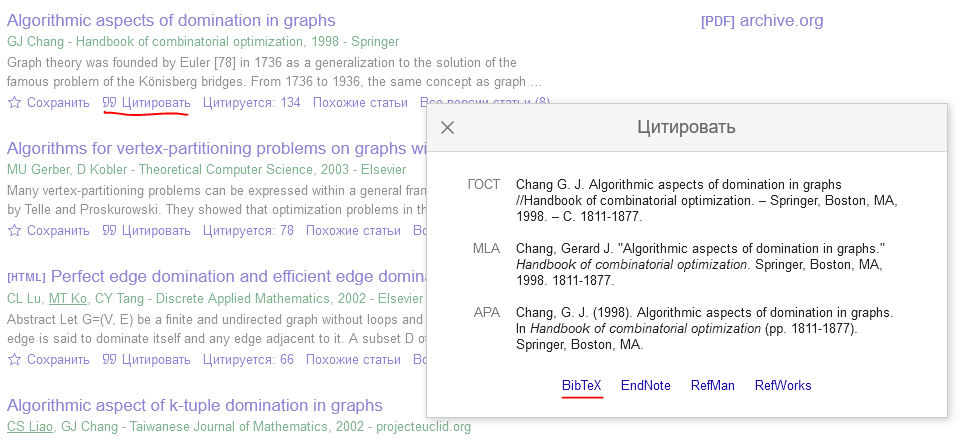
\includegraphics[scale=0.5]{res/img/scholar.png}
    \caption{Как получить bib-цитату на источник в Google Scholar.}
    \label{fig:scholar}
\end{figure}

Ссылка на источник происходит при помощи команды \verb|\cite|: \cite{duportail:alu}. В качестве единственного аргумента указывается идентификатор источника в одном из файлов \verb|*.bib|. Можно указать несколько источников: \cite{duportail:alu, husserl:pd, althusser:iia}, с \verb|\ref| так нельзя. В списке источников отображаются только те источники, на которых есть хотя бы одна ссылка. Если всё-же нужно что бы он там появился без единой ссылки, можно использовать команду \verb|\nocite| в любом месте программы, как под этим абзацем.

Вообще все ссылки кликабельны. Если ссылка неправильная, компилятор выдаст предупреждение, а ссылка будет выглядеть так: \textbf{??}.

\nocite{duportail:alu}
\nocite{althusser:iia}
\nocite{husserl:pd}
\nocite{husserl:sbe}

\chapter{Промышленная экология и безопасность}
\label{cha:bzd}

\section{Протестируем специальные символы.}

И заодно переключение шрифтов.

{\shorthandoff" \texttt{"-{}-* Прямая речь "-{}-{}- <{}<после ,{},тире`{}` неразрывный пробел>{}>}}

{\cyrillicfonttt{\bfseries\itshape\textbackslash{}cyrillicfonttt}
"--* Прямая речь "--- <<после ,,тире`` неразрывный пробел>>.}

{\cyrillicfontsf{\bfseries\itshape\textbackslash{}cyrillicfontsf}
"--* Прямая речь "--- <<после ,,тире`` неразрывный пробел>>.}

{\cyrillicfont{\bfseries\itshape\textbackslash{}cyrillicfont}
"--* Прямая речь "--- <<после ,,тире`` неразрывный пробел>>.}

\blindtext

\WhatAWrongCommand
\backmatter % здесь заканчивается нумерованная часть документа и начинаются ссылки и
            
\Conclusion

В результате проделанной работы стало ясно, что ничего не ясно...
 % заключение

\bibliographystyle{ugost2008}
\bibliography{references}


\appendix % тут идут приложения

\chapter{Картинки}
\label{cha:appendix1}

\blindtext

\begin{figure}
    \centering
    \includegraphics[scale=3]{example-grid-100x100pt}
    \caption{Картинка в приложении}
\end{figure}


\chapter{Еще картинки}
\label{cha:appendix2}

\blindtext

\begin{figure}
    \centering
    \includegraphics{example-image-golden}
    \caption{Еще одна картинка, ничем не лучше предыдущей. Но надо же как-то заполнить место}
\end{figure}


\end{document}
